\chapter{Inducción electromagnética}
La fuente de fem no es una batería, sino una estación generadora de electricidad.
La inducción electromagnética nos dice que un campo magnético que varía en el tiempo actúa como fuente de campo eléctrico.
También, un campo eléctrico que varía con el tiempo actúa como fuente de un campo magnético

\section{Ley de Faraday}
El flujo magnético total $\Phi_B$ a través de un área finita es la integral de esta expresión sobre el área:
\begin{equation}\label{29.1}
\Phi_B=\int\vec{B}\cdot d\vec{A}=\int B\, dA\cos\phi
\end{equation}
En el caso de que $\vec{B}$ sea uniforme sobre un área plana $\vec{A}$, entonces
\begin{equation}\label{29.2}
\Phi_B=\vec{B}\cdot \vec{A}=BA\cos\phi
\end{equation}
La \textbf{Ley de Faraday de la inducción} establece lo siguiente:
\textit{La fem inducida en una espira cerrada es igual al negativo de la tasa de cambio del flujo magnético a través de la espira con respecto al tiempo}.
 
En símbolos
\begin{equation}\marginnote{Ley de Faraday}\label{29.3.faraday}
\boxed{\varepsilon=-\frac{d\Phi_B}{dt}}
\end{equation}
\textbf{Obervación}: Las fem inducidas son ocasionadas por \textbf{cambios de flujo}.

Si se tiene una bobina con $N$ espiras idénticas y si el flujo varía a la misma tasa a través de cada espira, la fem total en la bobina es
\begin{equation}\label{29.4.Nfaraday}
\boxed{\varepsilon=-N\frac{d\Phi_B}{dt}}
\end{equation}
La \textbf{Ley de Lenz} establece que, \textit{la dirección de cualquier efecto de la inducción magnética es la que se opone a la causa del efecto.}
\section{Fuerza electromotriz de movimiento}
\begin{figure}[h]
\centering
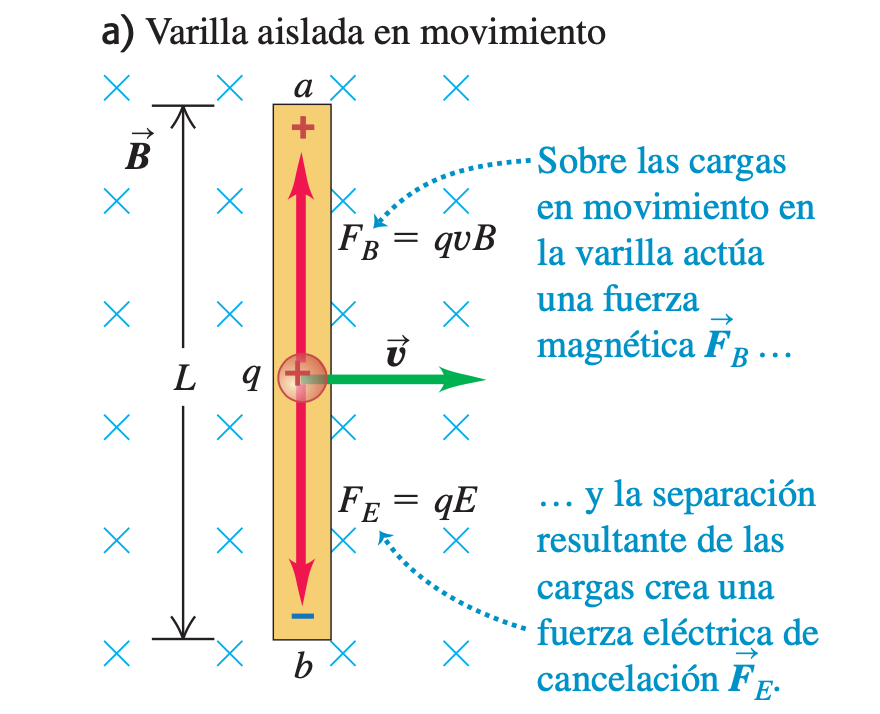
\includegraphics[scale=0.5]{fig/varilla}
\end{figure}
Una partícula cargada $q$ (	que suponemos positiva) en la varilla experimenta una fuerza magnética $\vec{F}=q\vec{v}\times\vec{B}$ con magnitud $F=|q|vB$. Esta fuerza magnética hace que las cargas libres en la varilla se muevan, lo que crea un exceso de carga positiva en el extremo superior $a$ y de carga negativa en el extremo inferior $b$.
Esto, a la vez, crea un campo eléctrico $\vec{E}$ en el interior de la varilla, en el sentido que va de $a$ hacia $b$ (opuesto al campo magnético). Llega un momento en el que $\vec{E}$ es lo suficientemente grande como para que la fuerza eléctrica ($qE$) cancele exáctamente a la magnética. De esta manera, $qE=qvB$, y las cargas están en equilibrio. Luego, se tiene que
\begin{equation}\label{29.5}
V_{ab}=V_a-V_b=EL=qBL
\end{equation}
con el punto $a$ a un potencial mayor que $b$.
\textbf{Continua...}
\subsection{Fem de movimiento: Forma general}
Podemos generalizar el concepto de fem de movimiento para un conductor de cualquier forma que se mueva en un campo magnético, uniforme o no (suponiendo que el campo magnético en cada punto no varía con el tiempo). Para cualquier fem cerrada, la fem total es
\begin{equation}\label{29.7}
\varepsilon=\oint (\vec{v}\times\vec{B})\cdot d\vec{l}
\end{equation}
Cuando se tienen conductores fijos en campos magnéticos cambiantes, no es posible utilizar la ecuación \ref{29.7}. En tal caso utilizar la ley de Faraday, ecuación \ref{29.3.faraday}.


\section{Campo eléctricos inducidos}
Una fem inducida también se presenta cuando hay un flujo cambiante a través de un conductor fijo.

\begin{figure}[h]\label{fig:galvanometro}
\centering
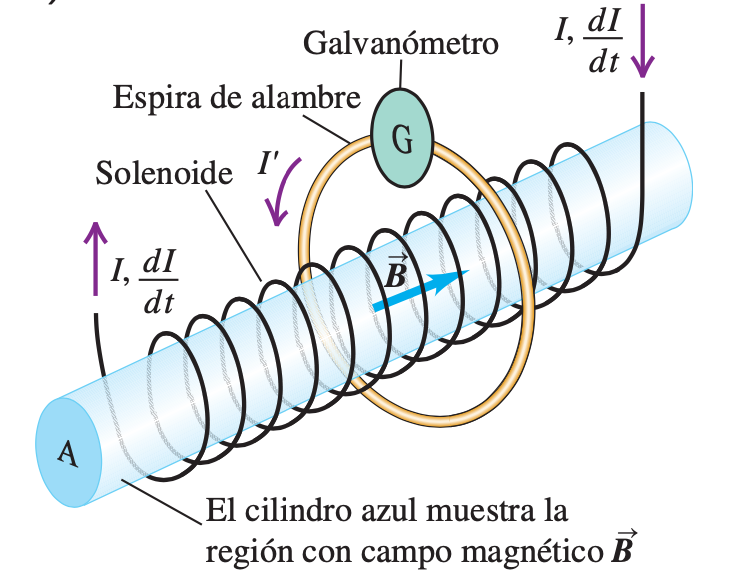
\includegraphics[scale=0.5]{fig/galvanometro}
\caption{El devanado de un solenoide largo lleva una corriente que se incrementa a una tasa $dI>dt$. El flujo magnético en el solenoide aumenta a una tasa $d\Phi_B/dt$, y este flujo cambiante pasa a través de una espira de alambre. En la espira se induce una fem $\varepsilon= -d\Phi_B/dt$, la cual induce una corriente $I'$ que se mide con el galvanómetro G}
\end{figure}

Consideremos la situacion que se ilustra en la figura \ref{fig:galvanometro}. Un solenoide largo y delgado, con área de sección transversal $A$ y $n$ espiras por unidad de
longitud, está rodeado en su centro por una espira conductora circular. El galvanómetro G mide la corriente en la espira. Una corriente $I$ en el devanado del solenoide establece un campo magnético $\vec{B}$ a lo largo de su eje, como se indica, con magnitud $B=\mu_0nI$, donde $n$ es el número de espiras por unidad de longitud. El flujo magnético a traves de la espira es $$\Phi_B=BA=\mu_0nIA$$ Cuando la corriente $I$ cambia con el tiempo se tiene, según la ley de Faraday

\begin{equation}\label{29.8}
\varepsilon=-\frac{d\Phi_B}{dt}=-\mu_0nA\frac{dI}{dt}
\end{equation}

Si la resistencia total de la espira es $R$, la corriente inducida en la espira es $I'=\varepsilon/R$. ¿Qué fuerza hace que las cargas se muevan alrededor de la espira? No puede ser una fuerza magnética porque el conductor no se está moviendo en un campo magnético, y en realidad ni siquiera está en un campo magnético. Se debe a un \textbf{campo magnético inducido} en el conductor \textit{causado por el flujo magnético cambiante}. Este campo eléctrico en la espira \textbf{no es conservativo}, porque la integral de línea de $\vec{E}$ a lo largo de la trayectoria cerrada no es igual a cero. En vez de ello, esta integral de línea, que representa el trabajo realizado por el campo inducido $\vec{E}$ por unidad de carga, es igual a la fem inducida $\varepsilon$:

\begin{equation}\label{29.9}
\oint\vec{E}\cdot d\vec{l}=\varepsilon
\end{equation}

Que según la ley de Faraday

\begin{equation}\label{29.10}\marginnote{Trayectoria de integración constante}
\boxed{\oint\vec{E}\cdot d\vec{l}=-\frac{d\Phi_B}{dt}}
\end{equation}

La forma de la ley de Faraday dada en la ecuación \ref{29.10}, sólo es válida si la trayectoria alrededor de la cual se integra es \textbf{constante}.

Un campo de esta clase recibe el nombre de \textbf{campo no electrostático}. Este campo, a pesar de no ser conservativo, ejerce una fuerza $\vec{F}=q\vec{E}$ sobre una carga $q$. De esta manera, un campo magnético actúa como fuente de campo eléctrico de una clase que \textit{no podemos} producir con ninguna distribución de carga estática.

\section{Corriente de desplazamiento y ecuaciones de Maxwell}
De igual manera que un campo magnético que varía da lugar a un campo eléctrico inducido, un campo eléctrico variable, da lugar a un campo magnético.

\subsubsection{Generalización de la ley de Ampere}
Recordando la ley de Ampere, $$\oint\vec{B}\cdot d\vec{l}=\mu_0I_{enc}$$ Esta ley, expresada de esta manera está \textit{incompleta}.
\textbf{continua...}







%\end{document}
